HTSLAM models the map as a hybrid topological-metric structure: the
environment is divided into a number of regions, and a local metric
map is built for each region. The relative poses of the regions are
stored in a topological structure. There is no global reference
frame. Only relative poses of the nearby regions are stored.

The motivation for the structure comes from a few sources. First,
dividing the world into a set of local maps appears to approximate the
way that humans reason \cite{psycho_kuipers82}. Second, is to ensure
that the mapping scheme scales to large environments.  The scalability
limitations of a single map SLAM methods are well known
\cite{guivant03,guivant01,guivant02} and prohibit real-time SLAM for
maps of practical size.  The third and final motivation is that a
robot does not require a single, global, metric description of the
world.  For example, in the ``fetch me a beer from the refrigerator''
task, there is no need for the robot to know the position of the
fridge while it is in the living room.  The robot only needs to know
the position of the fridge when it is near to the fridge.

This chapter describes the HTSLAM approach to map modelling.  Some
aspects of the map design are motivated by the mapping procedures
developed in chapter~\ref{chpt:Mapping} and so may only become fully
clear after reading chapter~\ref{chpt:Mapping}. The following section
describes the overall map structure.  Section~\ref{sec:local_map}
presents the methods used for modelling uncertainty within each local
map and section~\ref{sec:link} describes the methods used to model the
uncertainties of the topological links between maps.  Finally,
section~\ref{sec:region} discusses methods for defining the shape and
extent of each local region.

\section{Hybrid Map structure}
\label{sec:HM_structure}

\begin{figure}
\begin{center}
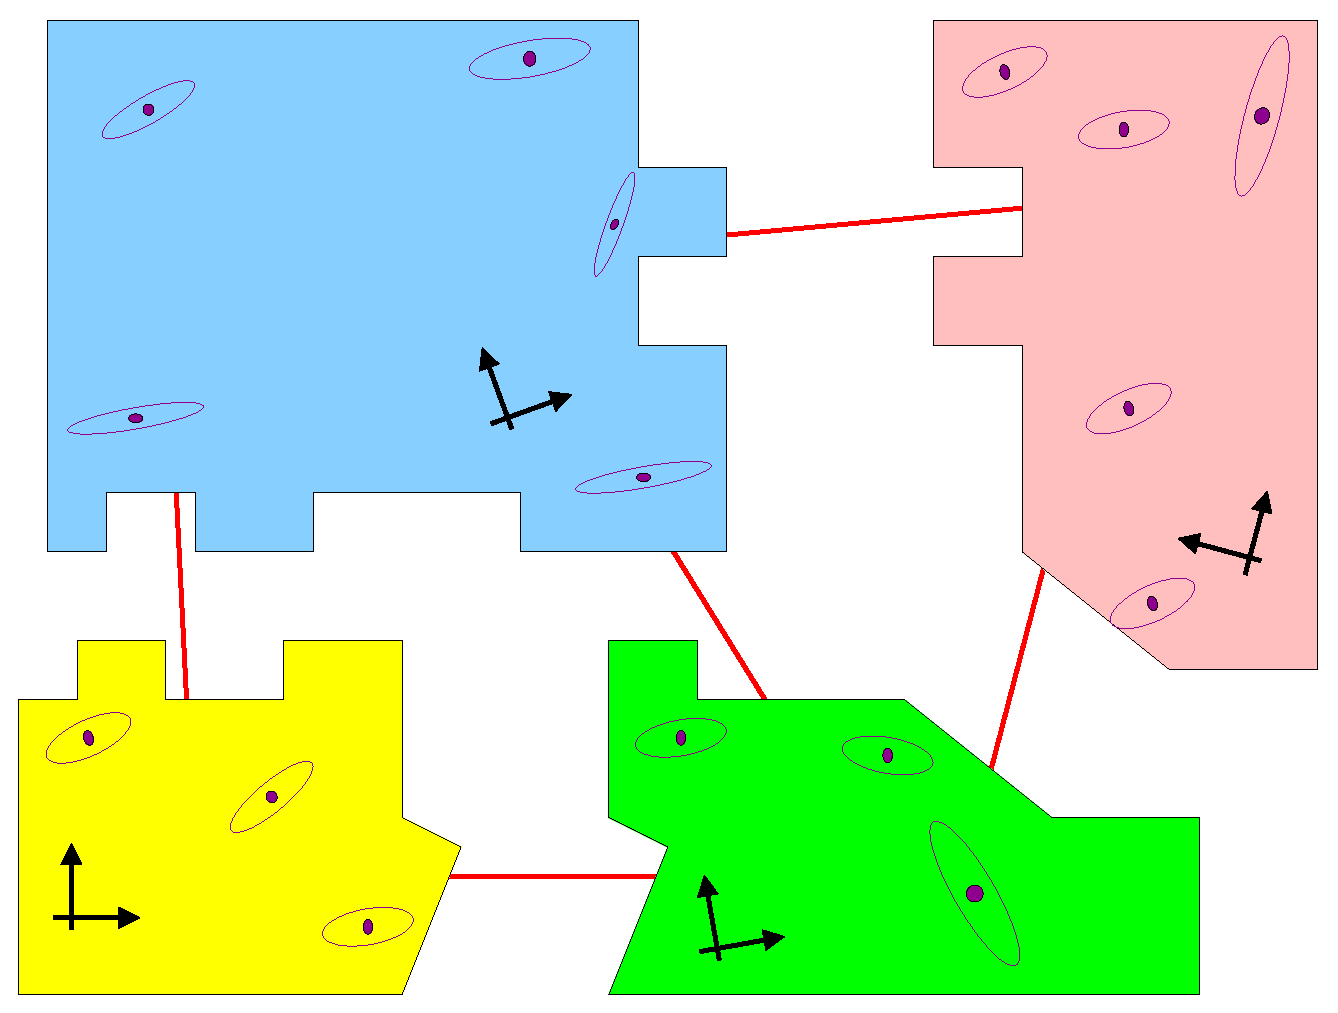
\includegraphics[width=10cm]{Pics/fig_map_structure}
\end{center}
\caption[Overview of HTSLAM map structure.]
{Overview of HTSLAM map structure. Each region has it's own
coordinate frame. The local map is built for every region (ellipses
erepresent landmarks). }
\label{fig:htslam_structure}
\end{figure}

\begin{figure}
\begin{center}
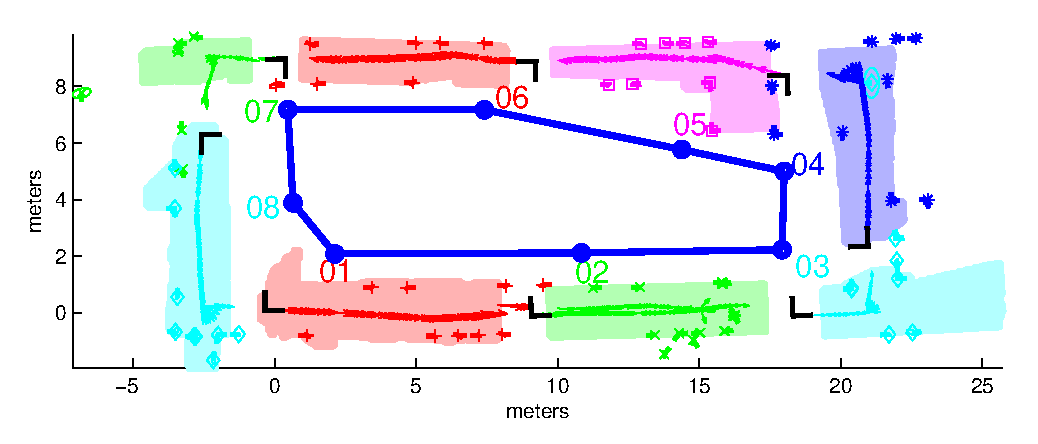
\includegraphics[width=14cm]{Pics/map_example_indoor}
\end{center}
\caption{Example of HTSLAM map for indoor environment}
\label{fig:htslam_structure_indoor}
\end{figure}


\begin{figure}
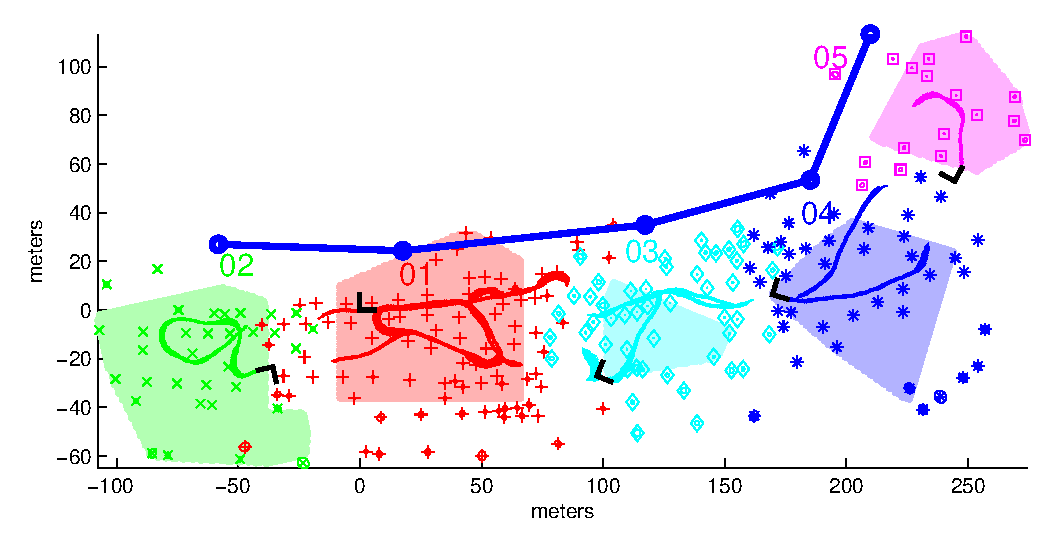
\includegraphics[width=14cm]{Pics/map_example_outdoor}
\caption{Example of HTSLAM map for outdoor environment}
\label{fig:htslam_structure_outdoor}
\end{figure}

In HTSLAM, a map is a connected graph. Every node of the graph
corresponds to a region within the environment. Each node has its own
reference frame and stores a local, metric map of the region and some
representation of the extent of the region in the local coordinate
frame. An example of HTSLAM map is given in the
\refFigure{fig:htslam_structure}. Note that there is no global reference
frame. The edges of the graph represent the stochastic coordinate
transformation between adjacent local maps
only. \refFigure{fig:htslam_structure_indoor} shows an example of an
HTSLAM map for indoor environment, and
\refFigure{fig:htslam_structure_outdoor} for an outdoor environment.

The structure used in HTSLAM is similar to that of \Atlas\
\cite{bosse02atlas}, however HTSLAM uses different uncertainty
representations, both for the coordinate transformations between
adjacent map frames and for the local maps.  \Atlas as a framework
allows to use arbitrary mapping model, however the two implementations
that have been published include EKF SLAM and scan matching.  \Atlas\
models the links or transitions between maps as Gaussian, and
therefore requires that the spatial uncertainty of the mapping module
is represented as a Gaussian.  On the other hand, HTSLAM uses
Rao-Blackwellised particle filter for the local maps (like FastSLAM),
permitting multi-modal modelling of the local map. HTSLAM also models
the transitions between maps using sets of particles.

A further difference between \Atlas\ and HTSLAM is that HTSLAM
maintains map extent information for every local map. This extra data
allows HTSLAM to perform map transitions and loop closing in a more
elegant way (as will be discussed later in
Chapter~\ref{chpt:LoopClosing}). In addition, HTSLAM explicitly
models the multiple hypotheses that arise during mapping, including
during loop closing, giving a more intuitively appealing and robust
approach.

The details of the uncertainty representation, both for each local map
and for the transitions between maps are discussed in the next two
sections.  Section~\ref{sec:region} discusses methods for
determining the extents of each local map.

\section{Modelling Uncertainty within a Local Map}
\label{sec:local_map}

To understand how uncertainty is represented within the local map, one
needs to be familiar with FastSLAM \cite{Montemerlo02d}, the mapping
scheme we use. An overview of FastSLAM was presented in
chapter~\ref{chpt:Overview}. In short, FastSLAM uses particles to
sample the possible paths of the robot. A map is built for each
path. Particles are evaluated based on how well the measurements match
the map.  Regular resampling is used to prune out unlikely paths.

The state $\s{k}{a}{m}$ of the $m$-th particle in the local map $a$
at time $k$ consists of the path of the particle within this local
frame, denoted \Xall{k}{a}{m}, and the map of the local environment
conditioned on the path, denoted \map{k}{a}{m}, i.e.
\begin{eqnarray}
 \s{k}{a}{m}    &=& [\Xall{k}{a}{m}, \map{k}{a}{m} ]\\
 \Xall{k}{a}{m} &=& [\x{0}{a}{m}, \x{1}{a}{m}, ... \x{k}{a}{m}]\\
 \map{k}{a}{m}  &=& [\mape{a}{m}{1}, \mape{a}{m}{2}, ..., \mape{a}{m}{n}],
\end{eqnarray}
where $\x{k}{a}{m}$ is the pose of a robot for the $m$-th particle at
time step $k$ in local map $a$ and $\mape{a}{m}{n}$ is the position of
an $n$-th landmark in local map $a$. The landmark position is a
stochastic variable, described by a Gaussian distribution. Note that
one does not have to store the whole path of a particle, since only
the most current pose of the particle is used in the mapping process.

A map is a probability distribution
$p(\map{k}{a}{m}|\Xall{k}{a}{m},\Zall{k}{a})$. If one makes an
assumptions that the map consists of landmarks, and that observations
are independent, then one can represent a map as a set of independent
landmarks, each conditioned on the path of a particle
$p(\mape{a}{m}{}|\Xall{k}{a}{m},\Zall{k}{a})$ (note that there is a
different map for each particle). FastSLAM approximates
$p(\mape{a}{m}{}|\Xall{k}{a}{m},\Zall{k}{a})$ with a Gaussian.  For
point landmarks, the distribution is a two-dimensional Gaussian
(location of the landmark on the plane). However, other landmark
characteristics can also be incorporated into the stochastic
variable. For example, if one builds a map of trees, the landmark
might have one extra parameter for the diameter of the tree trunk.
Note that since there are multiple particles, the actual posterior
distribution of the landmark is more complex than just a Gaussian. In
this thesis we will confine ourselves to planar motion. The results
however can be readily extended to full three-dimensional motion. Note
that, since the landmarks are estimated independently (in FastSLAM),
there is no need to maintain the global covariance matrix for the
whole map.

Each particle makes its own data association decisions. As a result,
the FastSLAM captures not only the uncertainty arising from the
continuous variables like robots' pose and the sensor measurements,
but also uncertainty due to discrete data association decisions.  This
uncertainty is not represented in the EKF approaches \cite{ekf_slam}.
The ability to capture this uncertainty is a big advantage, since in
most real-life situations the data association is ambiguous.

When mapping of a given local map is complete, the maps of all
particles alive at the time are stored within the local map. This set
of maps is effectively a sample from all the possible maps, given the
observations and odometry during the time robot was in the region.
Due to use of importance sampling, the sample from the maps is
expected to contain the most probable paths and their associated maps
(which are expected to be the better maps).

\section{Modelling Link Uncertainty}
\label{sec:link}
%Uncertainty of transformations

\begin{figure}
\begin{center}
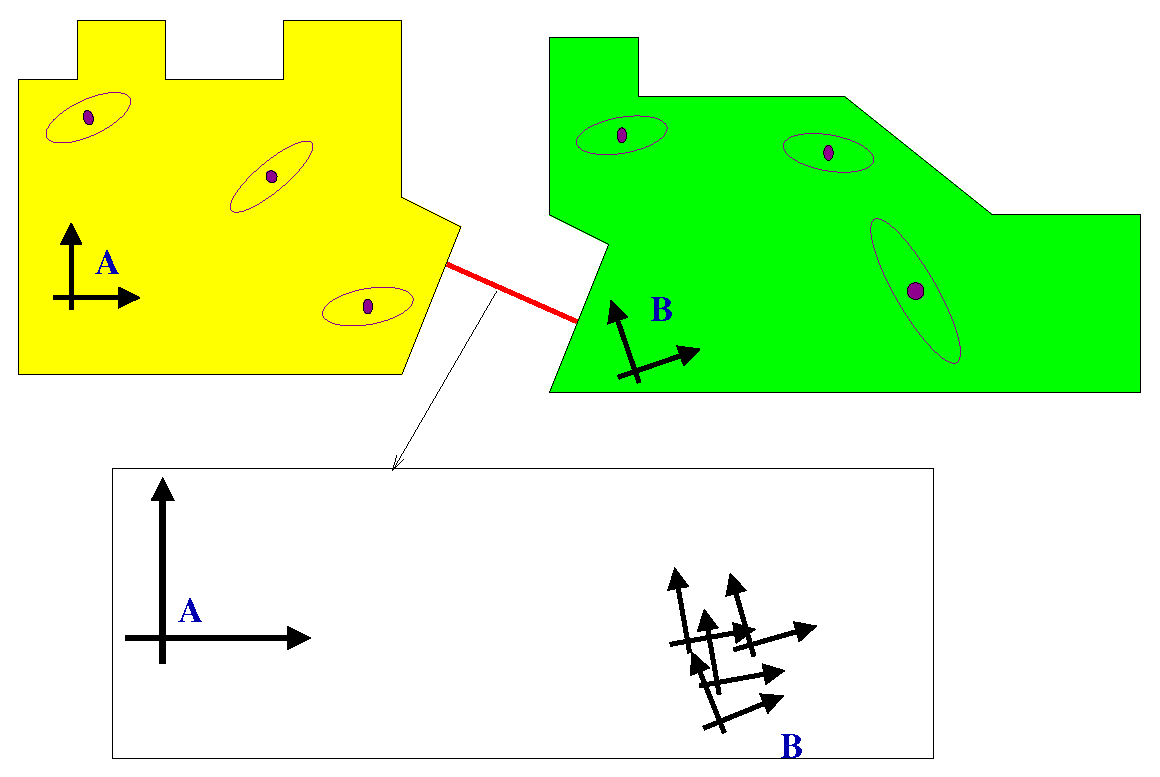
\includegraphics[width=10cm]{Pics/fig_transition_model}
\end{center}
\caption[Modeling transition distribution]
{Relative locations of the adjacent maps are represented by a
  set of particles.}
\end{figure}

The spatial relationships between adjacent local maps are each
represented by a set of particles.  As is common in SLAM
implementations, whenever a new map is started, the assumption is made
that the current location of the robot is precisely known in the new
map's coordinate frame.\footnote{Often it is assumed that the robot is
at the origin.  Here the position of the robot is chosen to place the
origin of the coordinate frame suitably for describing the local map
extents.} Thus, the transition between the old and the new map can be
most directly computed from the estimate of the robot pose in the old
map (a set of FastSLAM path particles) and the pose in the new map
(known by assumption). The transition is then a stochastic variable
which is most easily represented using particles. This is the chief
motivation for using a particle representation for the
transitions: the choice of representation makes the process of adding
new maps straightforward.

Note that when closing loops or, more generally, re-visiting maps,
there is no such easy method for transition determination and samples
must be taken from other distributions. For example, when closing
loops in HTSLAM, transition samples are taken from the results of map
matching (landmark matches are used to provide an estimate of
the transition function).

In general transitions and maps are not independent,
hence a joint probability needs to be stored. For adjacent maps $a$
and $b$ a joint probability distribution
$\prob{\map{}{}{a},\tr{}{a}{b}, \map{}{}{b}}$ is stored. Effectively,
the transition between the two adjacent maps captures a three-way
relationship between the two maps and the relative pose of the
reference frames of the two maps in a probabilistic manner. The exact
mechanism used to store the probability densities is described in more
detail in chapter~\ref{chpt:Mapping}.

It is worth noting that it is possible to derive the joint
probability $\prob{\map{}{}{a},\tr{}{a}{b},\map{}{}{b}}$ even for
non-adjacent maps $a$ and $b$ by merging probability densities along
the topological path joining the two maps.  The presence of loops in
the topological structure implies multiple paths between some of the
local maps. Therefore $\prob{\map{}{}{a},\tr{}{a}{b},\map{}{}{b}}$ can
be derived in several possible ways from the HTSLAM structure. This
adds a constraint to the HTSLAM structure, which will be discussed in
more detail in the chapter on loop closing(Chapter~\ref{chpt:LoopClosing}).

Let us define the coordinate transform using the \transit\ operator
\begin{equation}
\x{k}{}{b} = \x{k}{}{a} \transit \tr{}{a}{b}.
\end{equation}
This operator projects the pose of robot from one coordinate frame to
another.


\section{Defining Region Boundaries}
\label{sec:region}

Each region has its own ``area of influence''. This area is defined by
a grid map in the local reference frame. The size of the grid cells is
in the order of the robot's footprint, there is no need to have a
higher resolution. Regions who are neighbours in the topological
sense, have their region boundaries cropped in such a way as to
minimise the overlap. Grid maps are defined in local coordinates,
therefore one needs to transform grids from one reference frame to
another. Since relative poses of the neighbouring maps are known with
high certainty, the transformation is performed using the mean of the
relative poses of the two regions.

By limiting the area of the local map, the HTSLAM algorithm achieves
two major goals: firstly the computation requirements per local map
are bounded, since there is a finite number of landmarks in a finite
area, secondly the residual uncertainty of the robot pose within the
local region is bounded.


TODO: accentuate the difference in approach from Atlas, that
constantly monitors the pose uncertainty/performance of the
mapper/size of the map.

